\documentclass[preprint]{aastex}
\usepackage{amsmath,natbib}
%\usepackage{cite}
\usepackage{graphicx}
\usepackage[caption=false]{subfig}

%\setcitestyle{authoryear}
%\usepackage{cite}
%\documentstyle[natbib209]
%\citestyle{aa}
%\newcommand{\vdag}{(v)^\dagger}
%\newcommand{\myemail}{nkazmi2@illinois.com}
%{***YOUR EMAIL HERE***}

\shorttitle{Supernovae Iax Age Analysis}
%{***PUT AN SHORTENED TITLE HERE***}
\shortauthors{Kazmi, N. F. et al.}

\begin{document}

\title{Supernovae Iax Age Analysis}
%{***PUT TITLE HERE***}

\author{Novarah F. Kazmi\altaffilmark{1}, Ryan J. Foley\altaffilmark{1}, Curtis McCully\altaffilmark{2}}
\altaffiltext{1}{Astronomy Department, University of Illinois at Urbana-Champaign,
1002 W. Green Street, Urbana, Illinois 61801, USA.}
\altaffiltext{2}{Department of Physics, University of California, Santa Barbara, CA 93106}
%{Department of Physics and Astronomy, Rutgers, the State University
%of New Jersey, 136 Frelinghuysen Road, Piscataway, New Jersey
%08854, USA}
%\author{***FIRST AUTHOR'S LAST NAME, FIRST INITIAL MIDDLE INITIAL(?)***}
%\affil{***FIRST AUTHOR'S DEPARTMENT, INSTITUTION, CITY, STATE CODE ZIP 
%CODE***}
%\author{***SECOND AUTHOR'S LAST NAME, FIRST INITIAL MIDDLE 
%INITIAL(?)***}
%\affil{***SECOND AUTHOR'S DEPARTMENT, INSTITUTION, CITY, STATE CODE ZIP 
%CODE***}
%\author{***THIRD AUTHOR'S LAST NAME, FIRST INITIAL MIDDLE INITIAL(?)***}
%\affil{***THIRD AUTHOR'S DEPARTMENT, INSTITUTION, CITY, STATE CODE ZIP 
%CODE***}
%repeat as necessary

\begin{abstract}
\noindent We present an analysis of Supernovae (SNe) 2008ge, 2008ha, 2010ae, 
2010el. These SNe were observed using the Hubble Space Telescope (HST) in the
f435w, f555w, f625w, and f814w wavebands.  %optical wavebands.
These SNe are categorized as Type Iax, a distinct category from Type Ia or Type II. 
Type Iax are notable for their low spectra luminosity and low ejecta velocities. 
The stellar populations around these four SNe were analyzed to understand
 the ages of the SNe. In our study we examined the stellar populations
around each respective supernovae. We created color magnitude diagrams 
for each SNe and matched the sources to age isochrones. 
We found the ages for SNe 2008ge, 2008ha, 2010ae, 
2010el to be 19.5-27.5 Myr, 52.5 Myr, 22.4 Myr, 65.0 Myr respectively. 
These ages indicate a correlation between young stellar populations and
SNe Type Iax. 
%There is a correlation between the ages of the four separate SNe. 
%The details of the analysis include an examination of wavebands ; 
%adjusting the spectra for host and Milky Way (MW) reddening; 
%and filtering out sources with respect to their crowding, sharpness, and
% roub ndness features.
%%The occurance and trend in ages shows that IaX are a common feature
%% for all SNe.
% Further study needs to be done to have conclusive results. \\

%\smallskip
\noindent\textit{Key words}: supernovae: general - supernovae: individual (SN 2008ge, SN 2008ha, 
SN 2010ae, SN 2010el)%, SN 2012Z, SN 2014dt)
\end{abstract}

\section{Introduction}
A relatively new development in Supernovae (SNe) classification 
has been the Type Iax Supernovae (SNe Iax). 
These are separate from Type Ia SNe (no hydrogen lines, thermonuclear explosions) 
and Type II SNe (prominent hydrogen features, core-collapse), 
%SNe which are classified by their optical spectra then highlighted by the detonation mechanisms.
Iax are theorized to be thermonuclear explosions of Carbon-Oxygen
White Dwarf (C/O WD) and they share spectral properties with Ia SNe; however,
they have unique features which separate them from the traditional Ia SNe \citep{fol1304}. 

The differences between Ia and Iax begins with their luminosities.
Iax SNe possess a less luminous light curve, 
their absolute magnitudes fall between a range of 
``$-14.2 \leq M_{V,peak} \leq -18.4$ mag''
 \citep{fol1304}.
%The Iax rise-time rate is slightly larger than their Ia counterparts, 
%, a slow decline rate,
% NO CLEAR IDEA OF WHAT IS CORRECT FOR RISE/DECLINE RATE
%SOME ARE FAST, SOME ARE SLOW :\
The Iax lack an observable second maxima in the near-infrared (NIR),
which would be expected in Type Ia \citep{li03}. 
They have a lower ejecta velocity and do not show hydrogen and helium in their
 spectra.
The appearance of hydrogen and helium only occurs when there are environmental factors, such as  
a circumstellar disks or intermediate mass elements donating the material \citep{fol09}. 
Though the explosion mechanics of Iax are still unknown, the most accurate model
predicts a partial deflagration from the accretion of a Helium star 
onto a C/O WD \citep{krom13, fol1304}.

The host galaxies environments are significant because
the metallicity of the host galaxy affects the luminosity and the age of the
SNe explosion.
Iax have been identified in predominately late-time galaxies, 
but have not been observed in elliptical galaxies \citep{fol1304}. 
This is different from Iax, which are impartial to the galaxy type \citep{van92}. 
We would expect the SNe in more massive galaxies to have a brighter 
luminosity than SNe from smaller galaxies  \citep{fol1305}. 
Metallicity comes into play because progenitors with high 
metallicity results in lower luminosity light curves for their SNe \citep{tim03}. 
However, we know these from studies of Ia SNe, we can only vaguely frame Iax SNe with this information. 
%To truely understand the behaviors of Iax, we study specific parameters. 
 
%INCLUDE: Information about the affects host galaxies have on SNe.
%This will be useful when comparing the ages and seeing if the
%galaxies were important factors (metallicity and luminosity)

Though some parameters and features are known, there is still a lot 
that is not understood about Iax SNe.
The parameter that will be examined in this paper is the ages 
of the surrounding stellar population of these Iax.
By studying the ages of the remaining stars around the SNe,
we can predict the age of the Iax prior to detonation and 
see if there is a correlation of ages.  
%; however, SNe Iax are different from SNe Ia. 
%In the recent decade there has been an increase of SNe Ia analysis. 
%These studies reveal a range of behaviors and spectral features. 

In this analysis we study SN2008ge, SN2008ha, 
SN2010ae, and SN2010el. %, SN2012Z, and SN2014dt. 
The focus was on creating an age limit for the stellar populations around these SNe.
The stellar population around SN2008ha was analyzed in fig. 4 of \citet{fol1409}, 
the model recreated in this paper so as to apply the same method 
of analysis to SN2008ge, SN2010ae, and SN2010el. %, SN2012Z, and SN2014dt. 

In this paper, we will discuss our findings of Iax stellar populations.
% (this is a weird sentence).
In section 2, we will discuss the Spectroscopy and Photometry of these SNe .
%and compare them with earlier results. 
We will discuss members of the SNe Iax class in section 3. 
%We will discuss the methods of our analysis in section 3. 
In section 4, we will discuss methods.
The discussion of our results will be in section 5. 
The World Coordinate System (WCS) is used throughout this analysis. 
%Reddening shift of the Milky Way and host galaxies are used
%to measure the extinction of the spectra.

%(SNe Ia), have been studied in depth, 
%morose in the last decade due to the increase in technology and 
%an interest in the accelerating universe.
%Type Ia are used to measure the rate of expansion of the universe
%(Perlmutter et al. 1999) because of their near uniform light curves
%and relatively similar spectra. 
%However, not all thermonuclear explosions share this behavior. 
%Continued study of thermonuclear explosions reveal that they are not a "simple"
% category of SNe, they show a wide range of behaviors and spectral features. 
%Continued study of thermonuclear explosions reveal a range of behaviors 
%and spectral features. 


%The behaviors of SNe with peculiar features were cataloged as SNe Iax.
%The unique spectral features and low luminosity light-curves require a revised class
%thermonuclear explosions. 
%Therefore, SNe Iax are a separate category from SNe Ia.
%The unique features of Iax indicate that they are not a subset of Ia, 
%but should instead be considered their own class. 
%The differences between Ia and Iax indicate that 
%However, Iax are predicted to be a unique "set" of thermonuclear explosions. 
%While the mechanics of this model have not been finalized, 
%the spectra and light-curves of Iax show that it is a distinct type of SNe
%explosion, and not a subset of Ia. 

%Earlier literature called Iax, 'SN2002cx-like'. SN2002cx was examined
%because of it's [peculiar characteristics.] 
%The current class of Iax include 25 SNe.
%These SNe have a range of behaviors but do have low ejecta velocities, low light 
%curve luminosities, and lack the (usual) Ia features.  


\section{Spectroscopy \& Photometry}

This analysis used photometric images from the Hubble Space Telescope (HST) 
Advanced Camera for Surveys (ACS).
The SNe were observed in the F435W, F555W, F625W, and F814W wavebands. 
Data reduction was done by IRAF \footnote{IRAF (Image Reduction and Analysis Facility)
 is distributed by the National
Optical Astronomy Observatory, which is operated by the Association
of Universities for Research in Astronomy, Inc., under cooperative agreement
with the National Science Foundation.},  cosmic rays were removed using the L.A. Cosmic Algorithm,
the resulting images were used in the analysis. 

%This data was collected [DATE] using [type of collection method, ccd stuff,
%how the images were corrected]. 
%The HST collected these images using 
%(HST Info- exposures, camera lens size 
%and date and time it observed each object.
%I should include images of the SN discovery- tho not relevant)


\section{Class Members}
The catalog of SNe is growing and we are able to identify new SNe 
as Iax. Of the list of identified Iax SNe, we will focus on the following:  
SNe 2008ge, 2008ha, 2010ae, and 2010el. %, 2012Z, and 2014dt. 
SNe Iax have been observed in a variety of host galaxies, from S0 to spiral galaxies, 
though not elliptical galaxies \citep{fol09}. 
These different environments indicate another relation between the SNe. 
We will examining the environments around SNe 2008ge, 2008ha, 2010ae, and 2010el to 
to identify a trend in ages and SNe type. 
%The increase in new SNe data shows the variations in SNe spectra. 
%The classification of SNe was created when the data regarding Ia and II %
%SN showed unusual variations. 
%SN Iax are a result of the new classifications, Iax had a much lower
% light curve, (exact value), and other stuff ().  
%The current list of SNe Type Iax contain 25 SNe,
%of that list, 6 SNe were chosen to study in depth. 
% was determined to be a class Iax 
% Parameters

%2002cx and 2005hk were blue-shifted velocity ,
% 2008A red-shifted velocity because it had a unique velocity,
% this implies %that velocity shifts are unique for each SN
%5.  http://adsabs.harvard.edu/abs/2013arXiv1309.4457M

\begin{table}[htc]
\begin{center}
\caption{Supernovae Host Galaxies} 
\begin{tabular}{l*{6}{c}r}
\hline\hline
SN name & R.A. (J2000) & Dec. (J2000) & Host Galaxy  & Morphology & Reference  \\% &?  & ?\\
\hline
2008ge   & 04h 08m 24.686s & -47d 53m 46.93s    & NGC 1527           & SAB0$^{-r}$     & 1 \\%& ? &?\\
2008ha   & 23h 34m 52.652s   & +18d 13m 35.14s     & UGC 12682         &  Im                    & 1 \\%& ? &?\\
2010ae   & 07h 15m 54.698s   & -57d 20m 36.95s      & ESO 162-017  & Sb & 1 \\%& ? &?\\ %ESO 162- G 017  Sb? pec edge-on
2010el    & 04h 19m 58.816s   & -54d 56m 38.90s      & NGC 1566           & SABbc           & 1 \\%& ? &?\\ %SAB(s)bc 
%2012Z     & 03h 22m 05.3s   & -15d 23m 16s      & NGC 1309           & SA(s)bc             & 1 \\%& ? &?\\
%2014dt    & 12h 21m 57.57s  & +04d 28m 18.5s & M61 or NGC 4303 & SAB(rs)bc         & 1 \\%& ? &?\\
\hline
\end{tabular}
\label{tab:multicol}
\end{center}
\tablenotemark{{\bf References.}(1)}
%\tablenotetext{ALPHA TAG}{TEXT}
\end{table}
%(1) 
%RC3.9
%1991 vol. p. 
%DE VAUCOULEURS, G., DE VAUCOULEURS, A., CORWIN JR., H.G., BUTA, R. J. PATUREL, G., AND FOUQUE, P.
%THIRD REFERENCE CATALOGUE OF BRIGHT GALAXIES, VERSION 3.9 

\subsection{SN 2008ge}
\begin{centering}
	\begin{figure}
	\begin{minipage}[c][7cm]{.5\textwidth}
		\vspace*{\fill}
		\centering
		\includegraphics[scale = 0.50]{../Figures/SN08ge_Galaxy3.png}
			\label{fig:08gegal}
	\end{minipage}
	\begin{minipage}[c][7cm]{.5\textwidth}
		\vspace*{-.5cm}
		\centering
		\hspace*{1.48cm}\includegraphics[scale = .26]{../Figures/sn08ge_Region.png}
			\label{fig:r08ge}\par%\vfill
		\hspace*{1.45cm}\includegraphics[scale = .26]{../Figures/sn08ge_Source2.png}
			\label{fig:s08ge}
	\end{minipage}
	\caption{HST images of NGC 1527, host galaxy for SN 2008ge. We present a false color image,
	 F814W, F625W, and F435W, red, green, and blue respectively. \textit{Left: 200" x 135"}, NGC 1527,
	 the red box shows the position of SN 2008ge. \textit{Right-top: 10" x 10"}, 
	 this image refers to the red box on the left image. \textit{Right-bottom: 5" x 5"},
	This image refers to the white box from the above image. 
	Encircled is a .5" radius, corresponding to the location of SN 2008ge detonation.}
	\label{fig:08ge_whole}
	\end{figure}  
\end{centering}


The first observations of SN 2008ge were taken by
Chase on 2008 October 8.27 in NGC 1527 \citep{pig08}. 
NGC is a class SAB0$^{-r}$, S0, galaxy, a lenticular galaxy. 
SN 2008ge was observed after its maximum light, the observed peak was at
$M_{V,peak} = -17.4$ mag. %\citep{fol1011}.
 Previous observations of NGC 1527 do not show signs of star formation and a lack massive stars near 
position of the SNe, Fig.\ref{fig:08ge_whole} shows a similar observation.
This along with a ``large generated 56Ni mass all suggest a WD progenitor"  \citep{fol1011}.
There is no host galaxy reddening along the line of sight for SN 2008ge, however, there was 
Milky Way reddening, E(B-V) = 0.011. 


\subsection{SN 2008ha}

\begin{centering}
	\begin{figure}
	\begin{minipage}[c][8cm]{.5\textwidth}
		\vspace*{\fill}
		\centering
		\includegraphics[scale = 0.55]{../Figures/sn08ha_Galaxy.png}
			\label{fig:08hagal}
	\end{minipage}
	\begin{minipage}[c][8cm]{.5\textwidth}
		\vspace*{-.5cm}
		\centering
		\hspace*{-4.15cm}\includegraphics[scale = .27]{../Figures/sn08ha_Regions.png}
			\label{fig:r08ha}\par
		\hspace*{-4.15cm}\includegraphics[scale = .27]{../Figures/sn08ha_Source.png}
	\label{fig:s08ha}
	\end{minipage}
	\caption{HST images of UGC 12682, host galaxy for SN 2008ha. We present a false color image,
	 F814W, F625W, and F435W, red, green, and blue respectively. \textit{Left: 75" x 75"}, false color image of 
	UGC 12682, the white box shows the position of SN 2008ha. \textit{Right-top: 15" x 15"},
	This image refers to the red box on the left image. 
	\textit{Right-bottom: 2" x 2"}, This image refers to the rectangle in from the above image. 
	Encircled is the location of where SN 2008ha detonated.}
	\label{fig:08ha_whole}
	\end{figure}  
\end{centering}


SN 2008ha was first observed 2008 November 7.17 in UGC 12682, 
an Im type highly irregular galaxy, by POSS \citep{puc08}.
The first observations of SN 2008ha classified it as 
a SNe Ia with similar spectroscopic properties as SN 2002cx-like \citep{fol08}. 
At its peak SN 2008ha was observed with a $M_{V,peak} = -14$ mag, 
whereas SN 2002cx was observed at  $M_{V,peak} = -20$ mag. 
This puts SN 2008ha on the extreme end of this classification. 
It is less luminous and has one of the smallest ejecta velocity, ~3000$km/s$ lower than SN 2002cx. 
 \citep{fol09,fol1001,val09}.
We use use MW E(B-V) = 0.070 and no host galaxy reddening in this study. 
It was observed by the HST, it's false color image is presented in Fig.\ref{fig:08ha_whole}.
%An interesting character. It is an extreme case for IaX because of its low luminosity (-14.21 +/- .15 mag), slower ejecta velocity, KE, and Total Energy. Maybe had a massive progenitor. This SNe is discussed a lot, how come it wasn't made into it's own class. Compared with 2005E, however 2005E isn't IaX. 

\subsection{SN 2010ae}
\begin{centering}
	\begin{figure}
	\begin{minipage}[c][7cm]{.6\textwidth}
		\vspace*{\fill}
		\centering
		\includegraphics[scale = 0.5]{../Figures/sn10ae_Galaxy3.png}
			\label{fig:10aegal}
	\end{minipage}
	\begin{minipage}[c][7cm]{.5\textwidth}
		\vspace*{-.5cm}
		\centering
		\hspace*{-1.9cm}\includegraphics[scale = .26]{../Figures/sn10ae_Region.png}
			\label{fig:r10ae}\par
		\hspace*{-1.9cm}\includegraphics[scale = .26]{../Figures/sn10ae_Source.png}
			\label{fig:s10ae}
	\end{minipage}
	\caption{HST images of ESO 162-017,, host galaxy for SN 2010ae. We present a false color image,
	 F814W, F625W, and F435W, red, green, and blue respectively. \textit{Left: 80" x 55"}, false color image of 
	ESO 162-017,, the white box shows the position of SN 2008ha. \textit{Right-top: 10" x 10"},
	This image refers to the red box on the left image. 
	\textit{Right-bottom: 3" x 3"}, This image refers to the rectangle in from the above image. 
	Encircled is a .25" radius of where SN 2010ae detonated.}
	\label{fig:10ae_whole}
\end{figure}
\end{centering}

SN 2010ae was first observed on 2010 February 23 in ESO 162-G017, a spiral barred galaxy \citep{pig10}.
SN 2010ae was initially thought to be a SNe Ia; however, that classification
was redacted when analysis of its spectra showed strong similarities to
SN 2008ha. SN 10ae was then reclassified as SNe Iax \citep{str1003}.
We are observing ESO 162-G017 edge on, we are not sure of the locations of the neighboring stars
relative to the SNe detonation point. 
SN 2010ae, Fig.\ref{fig:10ae_whole} has Milky Way Reddening of E(B-V) = 0.008, as well as
host galaxy reddening of E(B-V) = 0.50 +/- 0.42 \citep{str1401}. 
%We will consider if these stars are in the foreground or if they lie in the same plane as the SNe.

%but these are all considerations we must make in order to understand our analysis.  
%In this analysis we will be looking at the stellar populations surrounding the SNe point. 


\subsection{SN 2010el}
%\begin{centering}
	\begin{figure}
	\begin{minipage}[c][7cm]{.6\textwidth}
		\vspace*{\fill}
		\hspace*{-1.5cm}\includegraphics[scale = 0.5]{../Figures/sn10el_Galaxy.png}
			\label{fig:10elgal}
	\end{minipage}
	\begin{minipage}[c][7cm]{.5\textwidth}
		\hspace*{-.3cm}\includegraphics[scale = .26]{../Figures/sn10el_Region2.png}
			\label{fig:r10el}\par
		\hspace*{-.3cm}\includegraphics[scale = .26]{../Figures/sn10el_Source.png}
			\label{fig:s10el}
	\end{minipage}
	\newline\caption{HST images of NGC 1566, host galaxy for SN 2010el. We present a false color image,
	 F814W, F625W, and F435W, red, green, and blue respectively. \textit{Left: 280" x 200"}, false color image of 
	NGC 1566 the red box shows the position of SN 2010el. \textit{Right-top: 10" x 10"}, This image refers to the red 
	box on the left image. \textit{Right-bottom: 2" x 2"}, This image refers to the rectangle in from the above image. 
	Encircled is the location of where SN 2010el detonated.}
	\label{fig:10el_whole}
	\end{figure}
%\end{centering}
SN 2010el, Fig.\ref{fig:10el_whole}, was first observed on 2010 June 19 in NGC 1566, 
an intermediate spiral galaxy \citep{mon10}. 
It was classified Type Iax because its
spectra resembled that of SN 2008ha \citep{bes10}.
SN 2010el has Milky Way reddening of E(B-V) = 0.008 and host galaxy reddening of 
E(B-V) = 0.8. 

%\subsection{SN 2012Z}

%SN 2012Z was first observed on 2012 January 29 in NGC 1309,
%a normal spiral galaxy, by LOSS.
%SN 2012Z was classified as Iax when initial observations of its spectra
%displayed properties similar to Iax (Cenko et al. 2012).

%\subsection{SN 2014dt}
%SN 2014dt was first found on 2014 September 29.8 in M61 (Nakano & Itagaki
%(2014) a). 
% It was quickly classified as Type Iax and soon after was  observed with the HST. 
%The HST was able to collect data soon after the initial discovery. ()

%9. http://adsabs.harvard.edu/abs/2014A%26A...561A.146S  
%Hα and [Nii] λλ6548, 6583 emission, 12 + log (O/H) = 8.40 ± 0.18 dex
%O3N2 method suggests an averaged local metallicity of 12 + log(O/H) = 8.34±0.14 dex, where again the quoted uncertainty includes measurement and systematic errors. These oxygen abundance metallicities correspond to 0.52 and 0.44 the known solar metallicity of ∼8.69 dex (Asplund et al. 2009), and so are consistent with the metallicity of the LMC.

\section{Methods}
We examined the stellar environments of SNe 
 2008ge, 2008ha, 2010ae, and 2010el 
to constrain the age the SN would have been prior to detonation. 
Catalogs of the surrounding stellar population 
were generated using DolPhot and HST photometric images. 
Using DolPhot we were able to extract sources from the HST images 
and put those sources in a catalog for each SNe. 
The catalogs included all star-like objects above
a signal to noise threshold, but not necessarily real sources, therefore the catalog had to be
filtered manually and through parameter constrains. 
The filters would include real sources over specific S/N thresholds, 
The parameters were adjusted for each SNe environment to extract real stars sources from the catalogs.

SN 2008ge was the only candidate that required special treatment in this analysis. 
The bright galactic nucleus made it difficult to identify sources and separate it from noise. 
In order to look at the region of space around the coordinates of the SN
we made a subtracted image for each of the wavebands, this was essential in
properly identifying star-like sources. 
The subtracted images were created by splitting the galaxy into four quadrants, and subtracting 
cross quadrants. 

The remaining SNe did not have the same issues as SN 2008ge and we were able to look at catalog
 and HST image directly. The objects in the catalog were then filtered their 
S/N, sharp, crowd, and round parameters, and by visual filters to identify real sources.

There was no host galaxy reddening for SNe 2008ge and 2008ha, however there was Milky Way reddening 
for SNe 2010ae and 2010el. We included both host galaxy and milky way reddening in our final analysis 
for the SN 2010ae and SN 2010el. 

%Other than SN 2008ge, we were able to use the reduced photometry to in the analysis of SN 2010ae and SN 2010el. 
%depending on the environment of the host galaxy. 
%The subtracted images are shown in Figures ~\ref{fig:r08ge} \& ~\ref{fig:s08ge}, 
%highlighted are the real sources from the catalog. 
%In our analysis we used the Milky Way reddening as well as the Host Galaxy reddening. 
%Only SNe 2010ae and 2010el had host galaxy reddening and MilkyWay reddening. 
%Using the new catalogs for SNe 2010ae and 2010el,
%real sources were identified, either through constraints on crowding, sharpness, and roundness,
%or through a visual examination. The results from this analysis will be discussed in the next section. 
\section{Discussion \& Results}


%The ages of the stellar population in our paper are in agreement with the earlier paper. 

%SN 2008ge was observed 6.55 arcsec away from the center of it's host galaxy,
%NGC 1527, a bright lenticular galaxy. 

SNe Iax are a new category of SNe, they include a wide range of SNe with unique parameters.
This analysis studied the ages of the stellar populations to see if age was 
a factor in differentiating SNe Iax from others. 
%The age of the host galaxies can be a factor which separates SNe Ia from Iax.
By creating CMDs for the neighboring stellar populations,
we are able to measure the ages of the stars in that region. 
This allowed us to estimate the age the SN would have been prior to its detonation. 

We examined the environment around SNe Iax. 
We modeled our analysis after a previous study of SN 2008ha from \citet{fol1409}. 
The \citet{fol1409} paper showed a color magnitude diagram (CMD), focusing on 
concentric regions of 75, 150, 225 pc (15, 30, and 45 pix ) around the SNe. 
With our catalog of stars, we were able to recover the same
results as \citet{fol1409}, shown in Fig.\ref{fig:08haCMD}.
We found the age to be 52.5 Myrs for the 
stellar populations around SN 2008ha. 

The age of SN 2008ge was constrained between high and low metallicity limits. 
Using those limits we evaluated the age to be between 19.5-27.5 Myr, Fig.\ref{fig:08geCMD}.
For SN 2010ae we found the age to be 22.4 Myr, Fig.\ref{fig:10aeCMD}. 
The final SN 2010el neighboring population was found to be 65.0 Myr old. 
We included the reddening vector to show the effects of dust extinction in Fig.\ref{fig:10elCMD}
From these results, there is spread of ages between Iax;
however, these estimations show SNe Iax to have relatively young ages. 
This information indicates that Iax come from young stars, though
our current set of data only includes 4 values. 
This gives a weak relationship which would be strengthened by recreating this analysis for the remaining SN Iax.
Further cataloging of Iax will add to the information we have and give us a better model for these types of SNe.
  
\begin{figure}[p]
	\centering
	\includegraphics[scale=0.5]{../Figures/SN08ge_Final.png}
	\caption{For SN 2008ge, we used a metallicity range to be between $Z = .02$ dex and $Z = .03$ dex, 
	$12 + Log(O/H) = 8.68$  and $12 + Log(O/H) = 8.85$ respectively for SN 2008ge  \citep{pro11}. }
    	\label{fig:08geCMD}
\end{figure}
\begin{figure}[p]
	\centering
	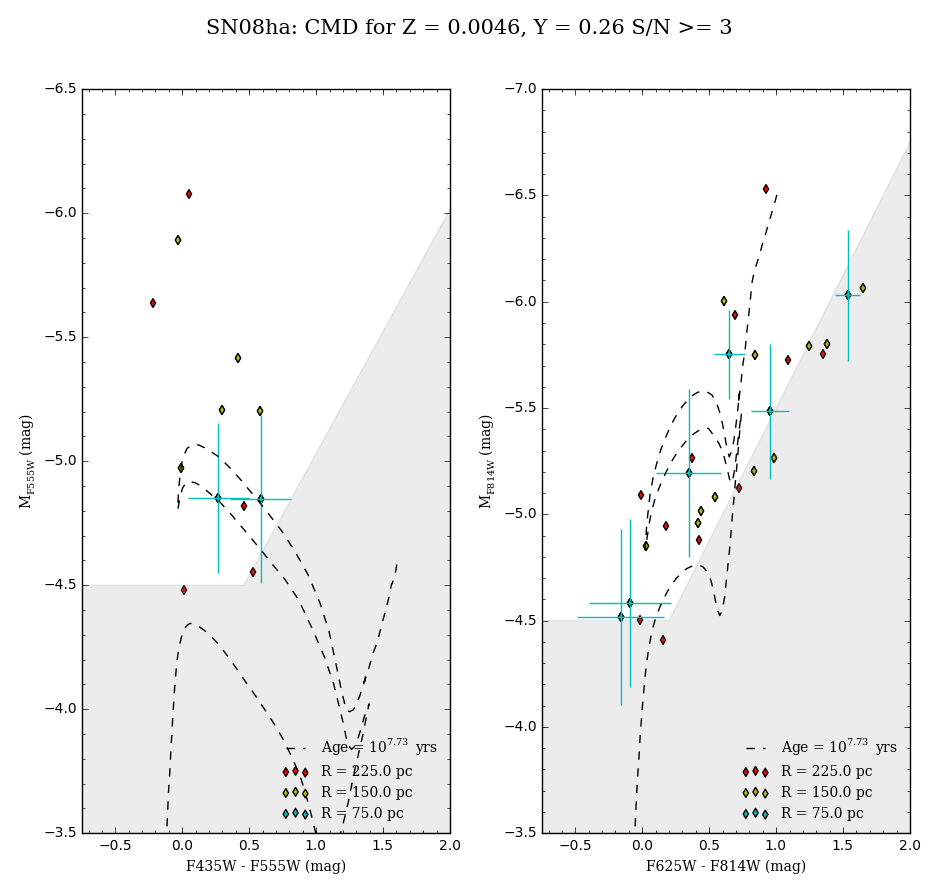
\includegraphics[scale=0.5]{../Figures/SN08ha_Final.png}
	\caption{SN 2008ha had an oxygen abundance of $ 12 + Log(O/H) = 8.16, Z = 0.006$ \citep{fol09,tak95}.}
    	\label{fig:08haCMD}
\end{figure}
\begin{figure}[p]
	\centering
	\includegraphics[scale=0.5]{../Figures/SN10ae_Final.png}
	\caption{SN 2010ae had a metallicity of $ 12 + Log(O/H) = 8.36, Z = 0.0096$. }
    	\label{fig:10aeCMD}
\end{figure}
\begin{figure}[p]
	\centering
	\includegraphics[scale=0.5]{../Figures/SN10el_Final.png}
	\caption{ SN 2010el was highly reddened by it's host galaxy, we included the reddening vector 
	to demonstrate the affects of the host galaxy on the stellar population. 
	This region had an oxygen abundance of $ 12 + Log(O/H) = 8.73, Z = 0.0224.$}
    	\label{fig:10elCMD}
\end{figure}

%Fig () shows the same sources from different wavebands being plotted
%and a similar age limit. 
%The remaining criteria included it's position, the filters included sources within a radius 
%100 pixels, though the physical distance is dependent on the SNe being discussed. 
%The other criteria was the Signal to Noise (S/N), at minimum, 
%sources had to be above S/N of 3 in at least one waveband. 
%The sources also needed to have particular Crowding values, for example, 
%clustered sources may included extended sources, which would not be "good" 
%sources. The sharpness and roundness was also taken into account. 
%The sharpness was set to [], and the roundness was set to []. 
%Using these parameters, we were able to recreate the Color Magnitude Diagram (CMD)
%of SN 2008ha, figure () from (Foley ...). This study focused on the stars within
% (15, 30, and 45 pix or 730, 1500, 2200 AU)
%There are different host galaxies environments and thus, different metallicity values. 

%The NGC 1527 is bright and identifying sources in the HST images was difficult
%The catalog was made of S/N fluctuations, which aren't as helpful as you would think.
%So the catalog was constrained as much as I could reasonably make it. 
%This meant looking at bright and dim stars (though saying they're stars is really
%pushing the definition because sometimes it was just a flucuation). 
%Following that was excluding objects that were within 25pix of the center
%of the galaxy. This space was not identified well in the catalog. 
%Using the subtracted images of the wavebands, we are able to see 
%details of what is happening near center of the galaxy. 
%After constraining parameters, such as S/N, crowd, sharpness, and roundness, 
%we also visually searched for sources from the remaining list. 
%Yes, super tiresome and really tedious. Oh well. 
%These steps took a region of space with over 1000 sources
%and reduced it to less than 30. 

%{\it Acknowledgments:} We are grateful to **ACKNOWLEDGEMENTS HERE***.

\bibliography{SNeIaxCite}{}
\bibliographystyle{apalike}
\end{document}